%\documentclass[11pt]{article}
\documentclass{article}
\usepackage[pdftex]{graphicx}
\usepackage{ifthen,fullpage}
\pagestyle{empty}



\setlength{\oddsidemargin}{0.25in}	% 1.25in left margin 
\setlength{\evensidemargin}{0.25in}	% 1.25in left margin (even pages)
\setlength{\topmargin}{0.0in}		% 1in top margin
\setlength{\textwidth}{6.0in}		% 6.0in text - 1.25in rt margin
\setlength{\textheight}{9in}		% Body ht for 1in margins
\addtolength{\topmargin}{-\headheight}	% No header, so compensate
\addtolength{\topmargin}{-\headsep}	% for header height and separation


% maximum fraction of page that can be a figure
\renewcommand{\dbltopfraction}{1.00}
\renewcommand{\topfraction}{1.00}
\renewcommand{\textfraction}{0.10}

% reduce enumeration spacing in a hacky way;
\newcommand{\itemvspace}{}%\vspace{-2mm}}
\newcommand{\postlistspacing}{}%\vspace{-0.08in}}

% reduce pre-pargraph spacing in a hacky way
%\newcommand{\preparagraphspacing}{}%\vspace{-0.15in}}
\newcommand{\preparagraphspacing}{\vspace{0.15in}}


\begin{document}

\begin{centering}
\section*{Tutorial: FPGA-SW Communication Using RRR and AWB}
\subsection*{Michael Pellauer}
\subsection*{Angshuman Parashar, Michael Adler, Joel Emer}
\end{centering}

\section{Introduction}

This tutorial introduces creating a FPGA-software hybrid system using Architect's Workbench (AWB) and Remote Request-Response (RRR). The reader should have
familiarity with basic AWB concepts and commands (in either the GUI or through the asim-shell command line). This tutorial covers:

\begin{itemize}
    \item Setting up an AWB workspace.
    \vspace{-7pt}
    \item Configuring, Building and Running AWB models (C++, Bluespec HDL, or hybrid).
    \vspace{-7pt}
    \item Creating a basic RRR specification for FPGA-software communication.
    \vspace{-7pt}
    \item Using RRR to build a working FPGA-software FIR Filter.
    \vspace{-7pt}
\end{itemize}

\section{Getting Started}

\subsection{Creating a Workspace}

To begin, let's create an AWB workspace to use for this tutorial. Having separate workspaces can help separate changes and make it easier to be working on several
different features at once. Name this workspace ``tutorial.''

\subsection{Readying your Workspace}

In your workspace, check out the ``hasim'' package. This package contains the files which let AWB configure and manage hardware-description language source code,
such as Bluespec (among other things). Also checkout the ``platforms'' packages, a useful library of functions for porting your design between a variety of
platforms, including different FPGAs. This package also contains an implementation of Remote Request-Response (RRR) protocol for FPGAs. This is our RPC-like
protocol for communicating between software and hardware, such as the FPGA.

\subsection{Explore your Workspace}

Notice the directories created AWB created in your workspace. These include:

\vspace{10pt}
\begin{tabular}{ll}
    \texttt{var/}                    & Directory for AWB to keep variables. You shouldn't need to alter this. \\
    \texttt{build/}                  & Configured models go here using symlinks into the \texttt{src/} directories.\\
                                     & We will use this for building and running models in the tutorial. \\
    \texttt{run/}                    & Directory for large experiment runs. We will not use this in this tutorial.\\
    \texttt{src/}                    & Source code for checked-out packages live in these subdirectories. \\
    \texttt{src/private/}            & This is an area for local (private, or unshared) files that you don't intend \\
                                     & to check into any package. We can put our source code we write for this \\
                                     & tutorial in this directory. \\
    \texttt{src/hasim/}              & Source code for the hasim package lives under this directory. \\
    \texttt{src/hasim/config/}       & Model configuration files (.apm) for a package live under this subdirectory. \\
    \texttt{src/hasim/modules/}      & Source code and AWB module descriptions (.awb files) live under this here. \\
\end{tabular}

\subsection{AWB Union Directories}

Note that AWB treats files and directory structures under the \texttt{src/<PACKAGE\_NAME>/} directories a little differently. These directories are conceptually
``unioned'' together into one namespace. For example, the contents of \texttt{src/hasim/config/pm/submodels/} and \texttt{src/platforms/config/pm/submodels/} are
combined into the tree \texttt{config/pm/submodels/}. You can test this using tab-completion in \texttt{asim-shell}. If you type ``configure package
config/pm/submodels'' and then hit TAB the contents of both directories will be shown in the tab-completion.

File name clashes from different packages should be avoided.

\section{Tutorial Project: FIR Filter}

Now that you're set up, let's do an example project. In this tutorial we will use a simple Finite Impulse-Response (FIR) Filter as a motivating example. You have
been provided code for two AWB FIR filter systems. The first, \texttt{bluespec/demos/fir\_filter\_sw}, is written exclusively in C++ and runs in software on the
host processor. The second, \texttt{bluespec/demos/fir\_filter\_hw\_exe} is written exclusively in Bluespec and represents hardware and a test harness to drive it.
Since a hardware description by itself with no inputs or outputs is pretty useless, we choose to simulate the hardware that represents. Hence the \texttt{\_exe}
extension, which shows that this model will be compiled into a Bluesim executable rather than an FPGA configuration file.

Your job is to combine the two designs into one hybrid hardware-software design. The hardware component will run on the FPGA and be
a FIR pipeline. The software component will do things that software is good at, like calculating the input, controlling the run, and
recording the results.

Note that for such a small project the FPGA is unlikely to beat a software implementation in performance, but the project is still
illustrative of the techniques you can use to build more complex projects.

\subsection{Filter Specification}

There are numerous kinds of FIR Filters, and numerous ways to implement each kind. For the purposes of this tutorial we will look at
an extremely simple 256-tap FIR Filter sequential pipeline:

\vspace{10pt}
\begin{centering}

    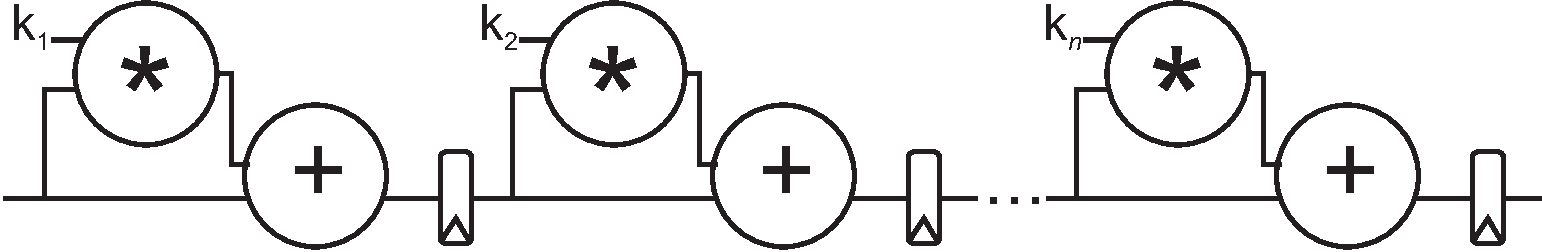
\includegraphics[width=0.80\textwidth]{FIRFilter.pdf}

\end{centering}

Where $k_1$ to $k_n$ represent user-settable coefficients. This pipeline is probably not the way a DSP expert would design it, but it is easy to describe and
illustrative for the purposes of this tutorial. Our pipeline will operate on 32-bit fixed-point numbers, with 16 bits on either side of the decimal place.

\subsection{Software Version}

To start, explore the source code for the software only model. Open the model up in AWB, right click on the ``SW-Only FIR Filter''
module, and select Edit. Note that this module contains a C++ implementation of an FIR Filter, as well as a small library of
fixed-point arithmetic. Examine the function \texttt{fir} which actually performs the FIR calculation pipeline shown above.

Note: To make things easier for the purposes of this tutorial the ``software only'' model is actually a hardware-software model with a Bluespec file representing
an empty hardware component. The ``hardware only'' model is similar: a hardware-software model with an empty software component. This eases the transition to a
true hybrid system for the purposes of this tutorial.

Now configure and build this model using AWB. Once you have built it, run it using the ``fir/sin'' benchmark and examine the file fir.out. It should contain a
sine wave-like curve of numbers between 255 and -255.

\subsection{Hardware Version}

Now take a look at the source code for the hardware version. This contains a Bluespec FIR filter, and a test harness that drives it. Note that the FIR Filter
represents a 256-stage pipeline. This is the strength of the FPGA: if we can keep the pipeline full, then in one clock tick it will perform 256
additions/multiplications. Even performing the calculation for a single pipeline stage for the host processor takes multiple instructions (loads, stores, branch
checks, etc).

Configure, build, and run this model on the same benchmark. Note: The output for the Bluespec version is a bit different from the software version. I suspect this
is due to differences in the fixed-point arithmetic implementations. Both outputs track the same sine wave nicely, so lets ignore these differences for now. If
anyone has a better explanation for why this happens, let me know.

\section{Creating a Hybrid Version}

You are now ready to create an FPGA-software hybrid version of this design. The hardware will be the FIR pipeline. The software will
calculate the input and coefficients, pass them to the FPGA, and record the results. We'll begin by simulating the FPGA component
using Bluesim. So the software process will be communicating with what it thinks is hardware, but is actually a simulation of
hardware. Once we've debugged this version we'll transition to running on the FPGA for real.

\subsection{Create Your Module and Model}

To start let's create a new AWB module representing this system. Make a directory in \texttt{src/private} called
\texttt{modules/system/fir-filter/hybrid}. Copy the files from the hardware-only system. Rename them as appropriate and change the
.awb file to reflect your new module.

Now we need to create a model which uses your source code. Copy the \texttt{fir\_filter\_hw\_exe} (or use ``Save As...'' in AWB). Since our initial version is
going to run using Bluesim, let's name the new model \texttt{fir\_filter\_hybrid\_exe}. Once you've copied the file, edit it in the AWB GUI and select your new
module. Note: You'll probably need to push the ``Refresh'' button to update AWB's database of known modules.

\subsection{Creating an RRR Specification}

To begin we need to create a .rrr file which describes the communication pattern between hardware and software. RRR gives us the ability to describe multiple
services, each of which can have servers either in software or hardware. For now let's make a single service, named FIR. This service should have two methods
hosted on the hardware, \texttt{setCoeff()} and \texttt{fir()}. To keep things simple, let's make \texttt{fir} a blocking call which always returns the output of
the pipeline, similar to the software-only FIR function. This won't result in good performance, but will be easy for us to get up and running in hardware.

Your job is to choose good type signatures for these methods. Note that it your .rrr file can \texttt{\#include} other files if you want access to nicer types than
UINT32 (although UINT32 can be made to work too). The model \texttt{bluespec/demos/rrrtest} has a good example of a .rrr file which you can build from.

Add the .rrr file to to your .awb module specification and reconfigure your model. Now when you build your model AWB will automatically generate some stub code to
make interfacing with RRR easier. These stubs will be re-generated any time you change the .rrr file, so you should only need to reconfigure once.

\subsection{Interfacing with RRR Client Stubs}

Our software is the RRR client which communicates with servers running on hardware. In order to support this AWB has generated some C++ code containing a client
stub. To use it we need to include \texttt{asim/rrr/client\_stub\_FIR.h}. Now we can instantiate a \texttt{FIR\_CLIENT\_STUB\_CLASS} within our
\texttt{SYSTEM\_CLASS}. This class has methods called \texttt{setCoeff()} and \texttt{fir()}, with the type signature you gave them in your .rrr file. Change your
software's \texttt{Main()} method to use those methods to calculate the FIR functionality. Note: our fixed point C++ class has \texttt{toInt()} and
\texttt{fromInt()} functions to aid in casting from fixed point to ints without changing data representation. This is convenient for transmitting data to Bluespec,
which can use the \texttt{unpack} function to convert a 32-bit number into a 16/16 fixed point.

\subsection{Interfacing with RRR Server Stubs}

Our Bluespec code needs to access the RRR server stubs in order to respond to requests from software. First let's include \texttt{asim/rrr/server\_stub\_FIR.bsh}.
This file defines an interface type named \texttt{ServerStub\_FIR}, and a module of that type named \texttt{mkServerStub\_FIR}. The methods are slightly different
than the software version. They're named \texttt{acceptRequest\_setCoeff()}, \texttt{acceptRequest\_fir()}, and \texttt{sendResponse\_fir()}. (RRR methods with
responses are broken into two Bluespec methods so that the hardware can take any number of clock cycles to respond.) For now let's create two Bluespec rules, one
for setting coefficients, and one to perform the FIR calculation and send back the response.

At this point you're ready to build and simulate your hardware using Bluesim. Note that this configuration uses UNIX pipes to communicate between the processes,
and is likely to have the worst performance of any versions in this tutorial. This setup is mostly useful for debugging the Bluespec using Bluesim's waveform
dumping and \texttt{\$display} functionality.

\subsection{Creating an FPGA Version}


Once your hardware component works its time to create a version that can be run on the FPGA. First copy the
\texttt{fir\_filter\_hybrid\_exe} model to \texttt{fir\_filter\_hybrid\_htg} (for HiTech Global, the makers of our FPGA platform).
Now we must alter this model a bit. First, switch the \texttt{fpgaenv} module from ``Hybrid Simulation Environment'' to ``Hybrid
HTG-v5-PCIe Environment.'' This includes all of the Xilinx scripts we need. You probably also want to change the default build
target from from ``exe'' to ``bit.'' This is done by setting the parameter \texttt{MAKE\_ALL\_TARGET} in the ``model'' module.

Now this model is ready to run on the FPGA. When you configure and build this new model, it will default to creating an FPGA bitfile. (This process can take a
while. For the purposes of this tutorial you may want to turn down the N\_TAPS parameter to something smaller simply to speed up this step.) In addition, the
benchmark \texttt{run} script will actually program the FPGA (or reset it if it is already programmed to the correct configuration). Setup the same benchmark you
ran before and confirm that you get the same output fir.out file as in simulation. 

How much faster is running on the FPGA compared to Bluesim simulation? For a small program like FIR, how does it compare in performance to the host processor?

\subsection{Challenge: Pipelined RRR Calls}

As mentioned earlier, blocking RRR calls are easy to write, but can result in low performance. (Consider that our simple FIR filter will not shift unless it
receives new input.) The final step of this tutorial is to create a non-blocking version of the RRR \texttt{fir} method (one that does not return a result). Then, 
use this to create a hybrid system that's better at keeping the hardware FIR pipeline moving.

One way to do this would be to have a new software RRR server called \texttt{reportResult}. Then the software could pump in input repeatedly, while a separate
server handles printing results into the output file. In order to do this you'll need to learn to interface with RRR software server stubs, and Bluespec client
stubs. Look at the \texttt{modules/bluespec/rrrtest} models for a good example of interacting with these stubs.

\section{Next Steps}

At this point you've successfully created a hardware-software design using RRR and AWB. We hope you'll want to go on to more explore advanced topics such using RRR
software servers, AWB dictionaries, or the Starter and Controller classes. Hopefully this has given you a taste of the potential FPGA-accelerators can achieve when
paired with good interfacing paradigms. Please feel free to contact me with feedback and questions at \texttt{pellauer@mit.edu}

\end{document}

